\RequirePackage[l2tabu, orthodox]{nag}

\documentclass[a4paper]{article}

\usepackage[UKenglish]{babel}

\usepackage[sc,osf]{mathpazo}
\linespread{1.05}         % Palatino needs more leading (space between lines)
\usepackage[T1]{fontenc}

\newcommand{\liningnums}[1]{{\fontfamily{pplx}\selectfont #1}}

\usepackage[utf8]{inputenc}

\usepackage{microtype}
\usepackage{ellipsis}

\usepackage{fixltx2e}

\usepackage{amsmath, amssymb}
\newcommand{\vect}[1]{\mathbf{#1}}
%\usepackage{mhsetup}
\usepackage{mathtools}
\DeclarePairedDelimiter\parens{\lparen}{\rparen}

\usepackage{graphicx}
\usepackage{svg}

\usepackage{float}

% prevents floats from crossing section boundaries
%\usepackage[section]{placeins}

\usepackage[hidelinks]{hyperref}

%\usepackage[separate-uncertainty, range-units = single, range-phrase = --]{siunitx}
\usepackage{siunitx}
\DeclareSIUnit{\astronomicalunit}{au}
\DeclareSIUnit{\year}{yr}

\usepackage{nth}

\usepackage{listings}

\usepackage{color}

\begin{document}
  \selectlanguage{UKenglish} % Is this necessary?

  \author{}
  \title{Computer simulation of Jupiter's Trojan asteroids}
  \date{April 2015}
  \maketitle

  \begin{abstract}
   
    The orbits of asteroids bound to Lagrange points 4 and 5 of the Sun-Jupiter
    system were simulated in two dimensions. A linear multistep method was used
    to solve the equation of motion. The stability of the region surrounding
    each point was assessed by observing how far an asteroid would `wander'
    from its starting position. An asteroid placed at the point itself was
    found to have a range of wander of \SI{0.14}{\astronomicalunit}; it
    travelled in a `tadpole' orbit because of the Coriolis effect. The stable
    region lies along and just outside Jupiter's orbit, with a width on the
    order of \SI{1}{\astronomicalunit}. A quadratic empirical relation between
    the planet's mass and asteroid range of wander was derived. For planet/sun
    mass ratios greater than 0.02 no stability at the Lagrange points was seen.
    This is consistent with previous analytical results.

  \end{abstract}

  \section{Introduction}
    % trojan asteroids observed leading / trailing jupiter
    % trojan asteroids lie at l4/5
    %  - five lagrange points (DIAGRAM)
    %  - all at maxima in effective potential, so appear unstable
    % specific detail on l4/5
    %  - coriolis force prevents asteroid from leaving; ends up in
    %    tadpole/horshoe orbit.
    %  - l4/5 stable iff mass ratio >> ~25 [greenspan]
    % aims of project / outline of following sections
    %  - numerically simulate behaviour of asteroids
    %     - is the coriolis effect enough to keep the asteroid from leaving?
    %     - specifically examine their range of wander
    %  - how big is the region of stability around the lagrange point? what is
    %    its shape?
    %  - what effect does the mass ratio have on the range of wander?

    The Greeks and Trojans are two groups of asteroids observed to lead and
    trail Jupiter's orbit of the Sun (Figure~\ref{fig:trojans}). They lie
    around the L\textsubscript{4} and L\textsubscript{5} Lagrange points
    respectively and inherit their names from heroes of the mythological war.

    \begin{figure}
      \centering
      \caption{The Greek and Trojan asteroids (green). \cite{asteroids}}
      \label{fig:trojans}
      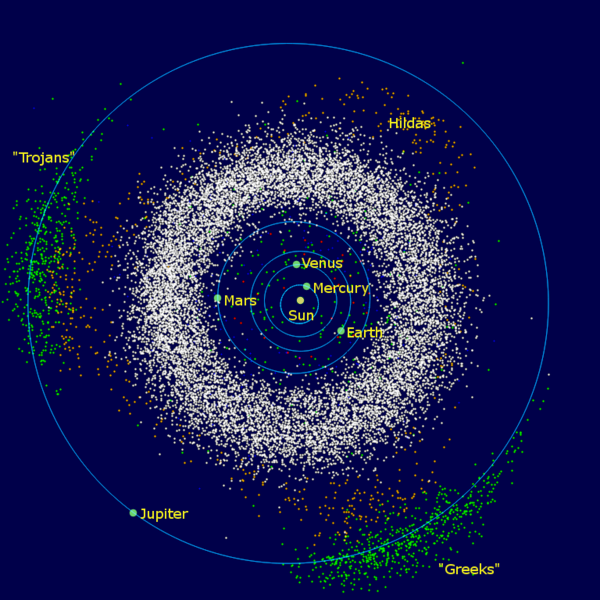
\includegraphics[width=0.8\textwidth]{figures/trojans}
    \end{figure}

    In a two body system, the five Lagrange points are those where the
    gravitational pull of the bodies is precisely equal to the centripetal
    force required for a third small mass to move with them. That is, a small
    mass placed exactly at one of the points should remain in stationary
    equilibrium with respect to the other two bodies. However, examining the
    effective potential (in the frame rotating about the barycentre ---
    Figure~\ref{fig:potential}) we see that these all occur at maxima and thus
    are not expected to be stable.

    So why, then, do L\textsubscript{4} and L\textsubscript{5} harbour
    asteroids in the Sun-Jupiter system? The answer is the Coriolis effect. As
    an object falls away from one of these points, the Coriolis force curves
    its path. If the ratio of the two large masses is much greater than 0.04
    then this deflection is actually significant enough to prevent the object
    from escaping \cite{greenspan}.

    \begin{figure}
      \centering
      \caption{Effective potential (rotating frame) of two bodies in
                orbit. The five Lagrange points all occur at maxima.
                \cite{wmap}}
      \label{fig:potential}
      \includesvg[svgpath=figures/,path=figures/,width=0.8\textwidth]{potential}
    \end{figure}

    The project described in this paper is a numerical simulation of the
    behaviour of the Trojan asteroids, confirming that they are indeed trapped
    about the \nth{4} and \nth{5} Lagrange points by the Coriolis effect. We
    will examine the range over which they deviate (or `wander') from the
    equilibrium point and thus infer the size and shape of the `stable' region
    around the Lagrange points.  We will also study the relationship between
    the planet's mass and the asteroids' range of wander.

  \section{Physical model}
    % simplifying assumptions
    %  - only examine one point. they are the same by symmetry [Marzari]
    %  - assume circular orbit of sun/planet around barycentre
    %    -> fixed R = 5.2; T = R^3/2 (in our system of units)
    %  - all lagrange points stable in z direction [greenspan 2014]
    %    -> examine 2d case in plane of orbit
    % equation of motion
    %  - ma = f + 2m(w x v) - m(w x (w x r))
    %       = f + 2mw(vy,-vx) + mw^2r (w perp r)
    %  - f = -gm(....) with rs = .... 
    % initial conditions
    %  - r0 = (rp - r/2 + dx, sqrt(3)/2 R + dy) (lagrange point plus offset)

    From a theoretical standpoint the dynamics of L\textsubscript{4} and
    L\textsubscript{5} are identical \cite{marzari}, so we need only focus on
    one of them. To simplify the problem we place the Sun and Jupiter in
    circular orbits about their barycentre such that they are at rest in our
    rotating reference frame (angular frequency $\omega$). Their separation is
    fixed at $R=\SI{5.2}{\astronomicalunit}$ with the other orbital parameters
    derived from this. In the direction perpendicular to the orbital plane, it
    can be shown that \emph{all} of the Lagrange points are unconditionally
    stable \cite{greenspan}.  Thus we restrict our attention to the two
    dimensions of the plane itself in order to investigate the particular
    overall stability of L\textsubscript{4} and L\textsubscript{5}.

    With these considerations, our asteroids obey the Newtonian equation of
    motion
    \begin{multline}
      \label{eq:motion}
      \ddot{\vect{r}} =
      - \frac{G m_s}{\parens*{(r_s+r_x)^2 + r_y^2}^\frac{3}{2}}
          \begin{pmatrix} r_x + r_s \\ r_y \end{pmatrix}
      - \frac{G m_p}{\parens*{(r_p-r_x)^2 + r_y^2}^\frac{3}{2}}
          \begin{pmatrix} r_x - r_p \\ ry \end{pmatrix}
      \\ + 2 \omega \begin{pmatrix} \dot{r}_y \\ -\dot{r}_x \end{pmatrix}
      + \omega^2 \vect{r}
    \end{multline}
    where $r_s$, $m_s$, $r_p$ and $m_p$ are the distances from the barycentre
    and masses of the Sun and Jupiter. The first two terms are the
    gravitational attraction of the bodies; the last two are the Coriolis
    and centrifugal forces respectively. The Lagrange point itself is given by
    $\vect{r}_0 = \parens{r_p - R/2, \sqrt{3}R/2}$.

  \section{Computer implementation}
    % scaling - solar system units
    %  - helps keep numbers reasonable and avoid numerical issues
    %  - unit mass = sun
    %  - unit distance = au
    %  - unit time = year
    % approach (and library routines)
    %  - write the equation of motion as four coupled first order ODEs:
    %     - drx/dt = vx, dry/dt = vy, dvx/dt = f(r,vy), dvy/dt = g(r,vx)
    %  - solve initial value problem using ODEPACK [hindmarsh]
    %     - linear multistep (like RK but use info from previous steps)
    %     - auto switches between Adams (non-stiff), BDF (stiff)
    %  - 'wander' as the furthest point on the trajectory from the lagrange
    %     point
    %  - run for 500 orbits, evaluating at min 100 points per orbit
    %  - parallel computation of trajectories
    %  - results saved to disk

    To keep numerical values in the simulation reasonable we work in the `solar
    system units' specified in Table~\ref{tab:units}. This diminishes any potential
    for arithmetic under/overflows.
    \begin{table}
      \centering
      \caption{Solar system units.}
      \label{tab:units}
      \begin{tabular}{r l}
        Quantity & Unit \\
        \hline
        Length & \si{\astronomicalunit} \\
        Mass & $M_{\odot}$ \\
        Time & \si{\year}
      \end{tabular}
    \end{table}

    The equation of motion (\ref{eq:motion}) may be re-written as four
    coupled first-order ordinary differential equations (ODEs):
    \begin{subequations}
      \begin{gather}
        \dot{r}_x = v_x \\
        \dot{r}_y = v_y \\
        \dot{v}_x = \dot{v}_x\parens{\vect{r}, v_y} \\
        \dot{v}_y = \dot{v}_y\parens{\vect{r}, v_x}
      \end{gather}
    \end{subequations}
    We now have form which can be solved by standard numerical techniques. In
    particular we employ a linear multistep method\footnote{Linear multistep
    methods keep and use information from previous steps; Runge-Kutta methods
    simply discard such data.} using the ODEPACK library
    routine LSODA \cite{hindmarsh}.

    As well as solving for the asteroid's trajectory we also compute its
    `wander'. This is the furthest distance it travels from the Lagrange point
    over the course of the simulation. It gives an indication of how tightly
    bound the asteroid is, i.e.\ its stability.

    Typically we simulate 500 Jupiter orbits, explicitly evaluating the
    asteroid position $\vect{r}$ at 100 points in each. These parameters were
    chosen to give acceptable precision whilst maintaining good performance.
    For the longer experiments, multiple processes (each solving a different
    set of initial conditions) were run in parallel. In some cases intermediate
    calculations were saved to disk so that subsequent minor tweaks did not
    necessarily incur a lengthy re-run.

    A number of simple test cases were examined in the process of validating
    the model and fixing bugs in the implementation. These sometimes consisted
    of fewer bodies, or included a subset of the forces.

    Appendix~\ref{app:code} contains the full source code in Python 3. The core
    routines are defined in Listing~\ref{src:lagrange.py}. The others are
    scripts which perform the actual experiments.

  \section{Experiments and Discussion}
    % - single run stability over many orbits
    % - plot of short run to show typical form of trajectory 
    %    - as expected l4/5 are not stable due to equilibrium; they are stable
    %      due to coriolis effect
    %    - remember that in the inertial frame the trajectory just looks like an
    %      ellipse which is slightly perturbed

    \begin{figure}
      \centering
      \caption{Stability over 5,000 Jupiter orbits. The asteroid's trajectory is
      denoted by the blue line; it remains confined to a small region around
      L\textsubscript{4} (marked by a cross). Sun and Jupiter not to scale.}
      \label{fig:single}
      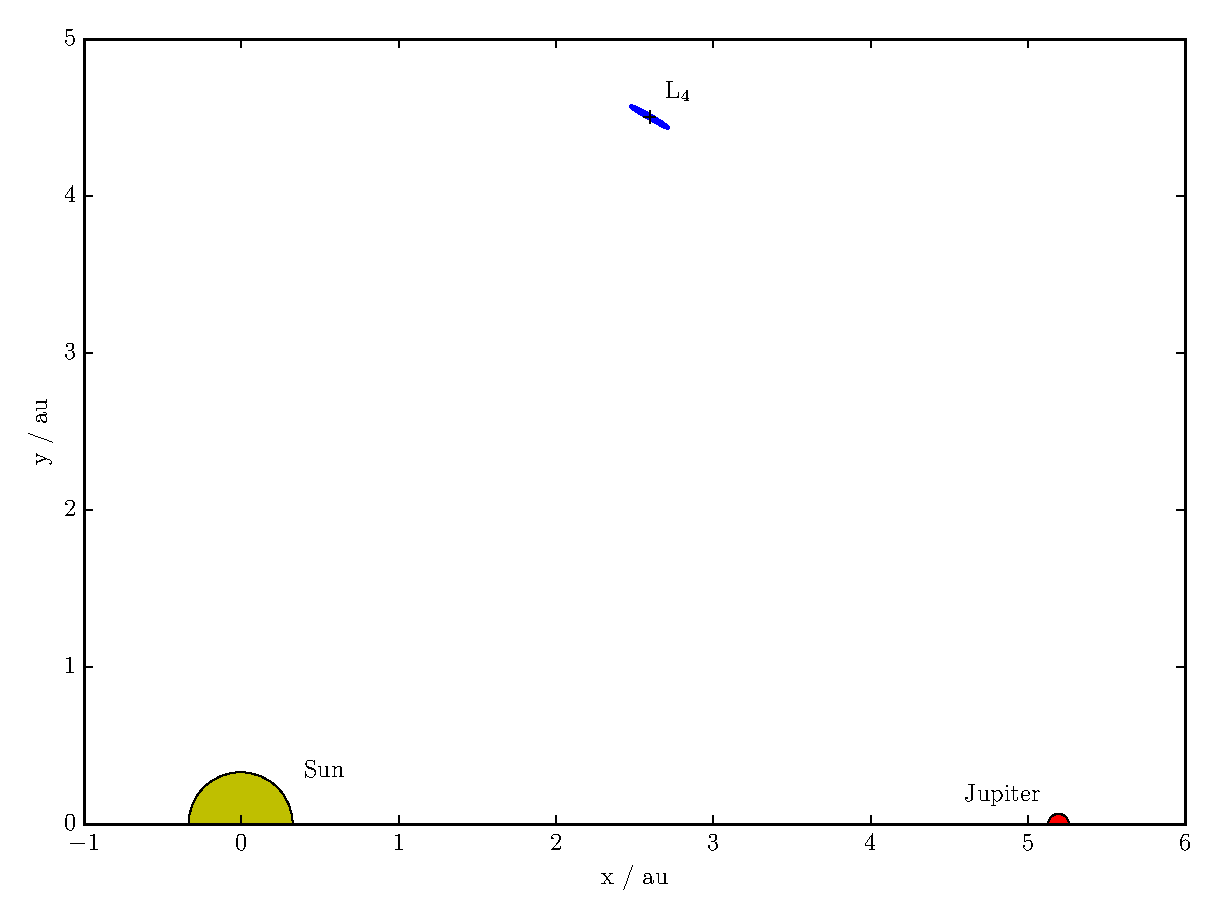
\includegraphics[width=0.8\textwidth]{figures/single}
    \end{figure}
    \begin{figure}
      \centering
      \caption{Asteroid trajectory over 12 Jupiter orbits. The starting point,
      L\textsubscript{4}, is marked by a cross.}
      \label{fig:typical}
      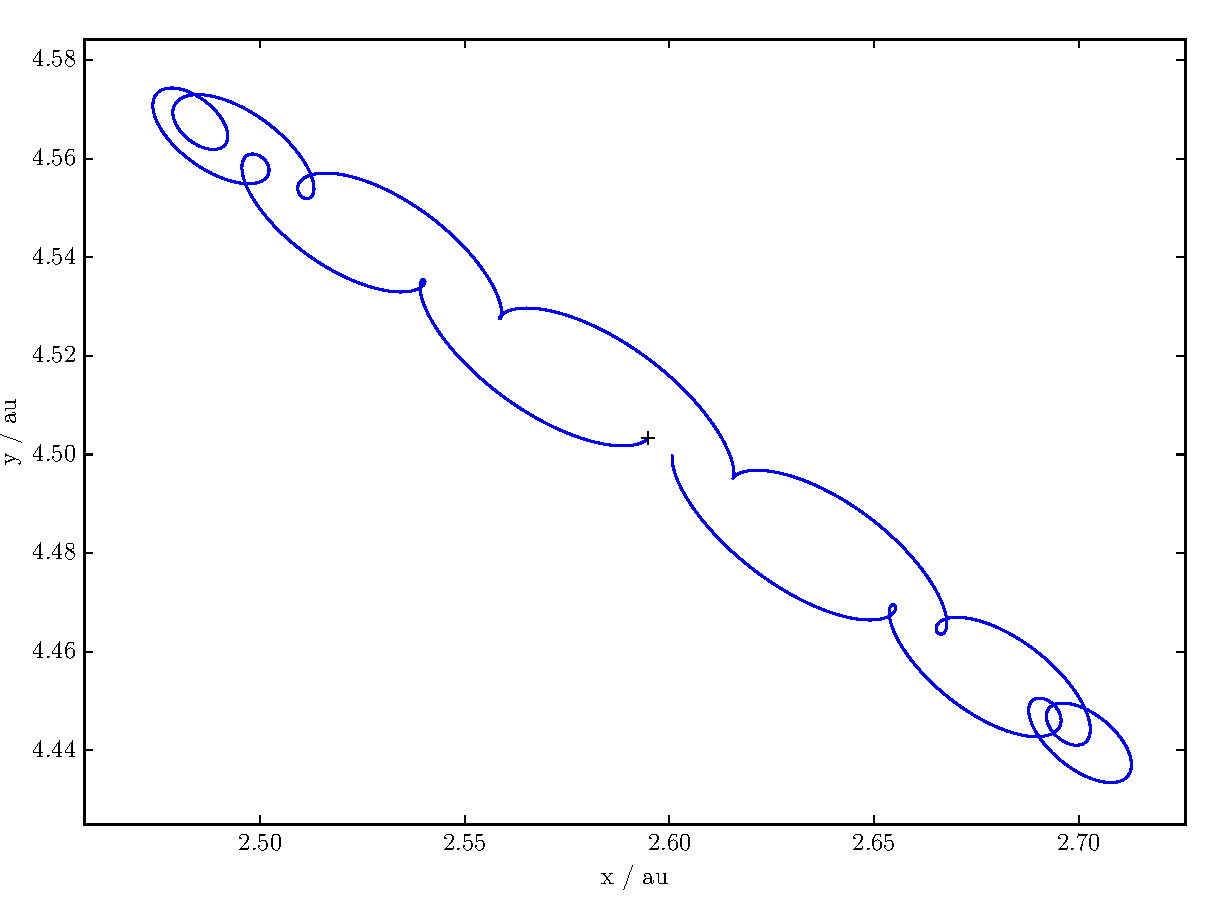
\includegraphics[width=0.8\textwidth]{figures/typical}
    \end{figure}
    Figure~\ref{fig:single} shows the result of running the simulation for
    5,000 Jupiter orbits. The asteroid was placed exactly (give or take
    numerical rounding) on the Lagrange point. The trajectory for the first 12
    orbits is detailed in Figure~\ref{fig:typical}. The range of wander in this
    case was \SI{0.14}{\astronomicalunit}.
    
    As expected the asteroid falls away from the Lagrange point; it is not
    in stable equilibrium. We see it follow a curved path due to the Coriolis
    effect, which prevents it from becoming free. The motion appears to contain
    two major components: a high frequency, small radius oscillation combined
    with a lower frequency, larger radius oscillation. The superposition gives
    the characteristic `tadpole' orbit typical of Trojan objects.

    It is important to remember that in the inertial frame these trajectories
    look far less convoluted. They are akin to an ordinary circular orbit which
    is being slightly perturbed.
    
    \subsection{Region of stability}
      \label{sec:regionofstability}
      % - method
      %    - place stationary asteroids on grid around lagrange point
      % - contourf plot 
      %    - offset.py: 141s to generate (-> 0.6 s / run)
      % - perturbing the asteroid along the line of the orbit has little effect
      %   on stability
      % - perturbing towards the sun has a slightly greater effect than away
      %   from
      %    - i.e. the most stable region is actually slightly outside jupiter's
      % - >0.06AU to/from sun results in loss of stability
      \begin{figure}
        \centering
        \caption{Range of wander as a function of starting position. The dotted
        line indicates Jupiter's orbit. The most stable region lies along
        and slightly outside of this.}
        \label{fig:offsetplot}
        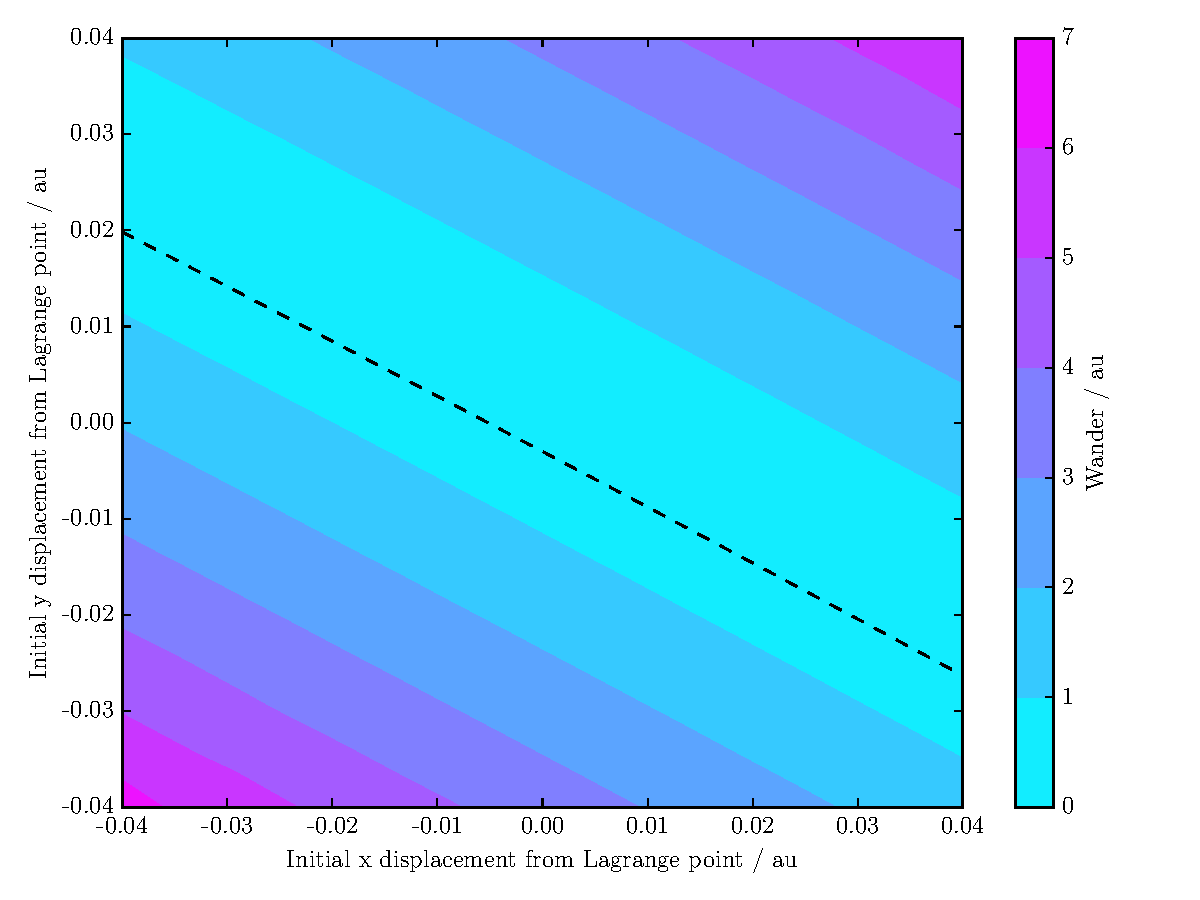
\includegraphics[width=0.8\textwidth]{figures/offset_plot}
      \end{figure}

      In order to investigate the stability of the area around the Lagrange
      point we run a number of simulations, each using a different asteroid
      starting point. The range of wander is thus calculated for each position,
      as shown in Figure~\ref{fig:offsetplot}. This result took
      \SI{141}{\second} to evaluate on an Intel Core \liningnums{i5} processor;
      that is \SI{0.6}{\second} per simulation run.

      Immediately we notice that the stable region has some shape. Perturbing
      the initial position along the line of Jupiter's orbit has very little
      effect, whereas in the perpendicular direction a small offset gives rise
      to a significant range of wander. Starting the asteroid more than
      \SI{0.06}{\astronomicalunit} to/from the Sun results in a total loss of
      stability. The shape here matches up with the asteroids' typical
      trajectories.  Notice also that the most stable region is actually
      slightly outside of Jupiter's orbit, not at the precise maximum of the
      effective potential.

    \subsection{Planet/sun mass ratio}
      \label{sec:massratio}
      % method
      %  - place stationary asteroid on lagrange point for each mass
      % line plot of mass vs wander
      % strong trend (+ve correlation)
      % masses above ~0.02 are not stable cf theory
      % very good fit to quadratic
      %  - linear contribution is biggest, then quadratic. constant negligible.

      \begin{figure}
        \centering
        \caption{Relationship between the planet's mass and 
        asteroid range of wander. A least squares fit yields the quadratic
        $3150 m^2 + 199 m + 0.05$.}
        \label{fig:mass}
        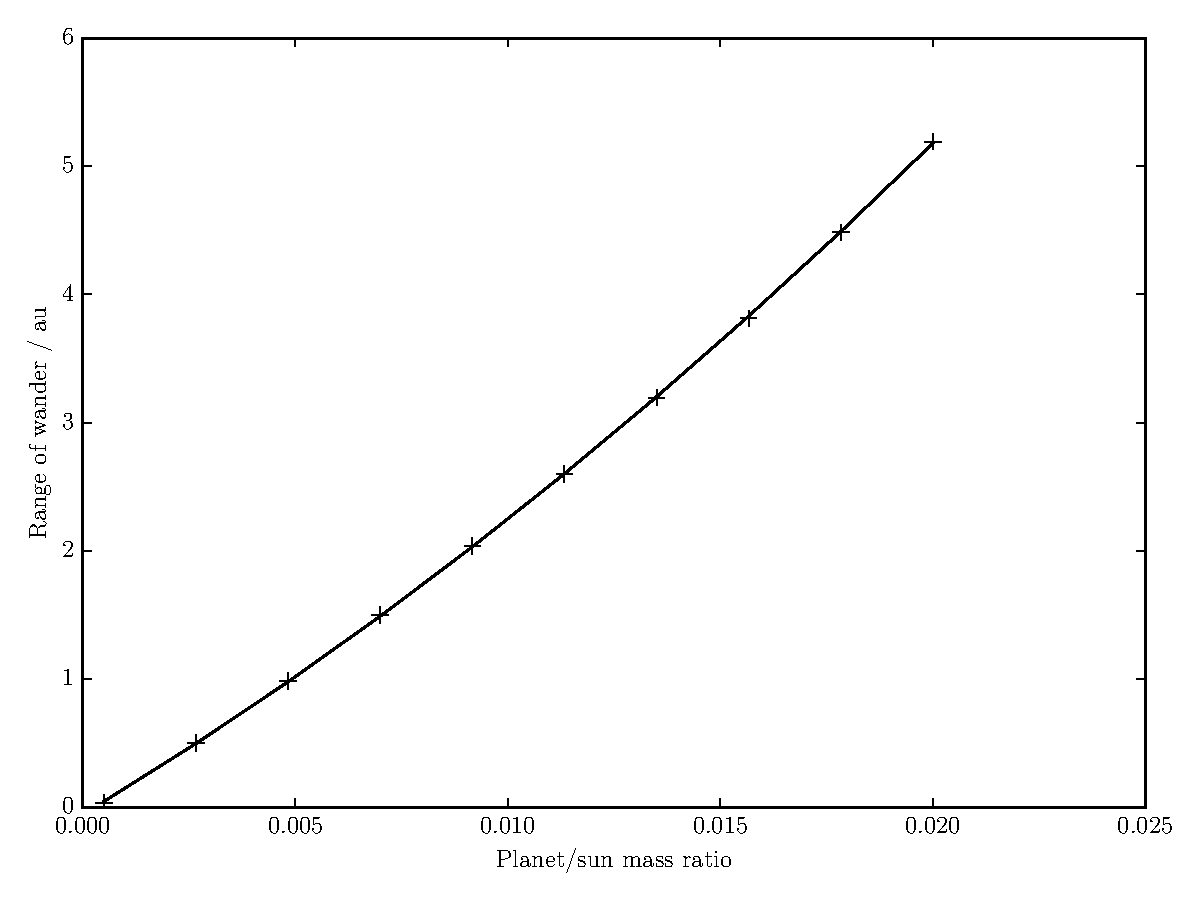
\includegraphics[width=0.8\textwidth]{figures/mass}
      \end{figure}

      Ten simulations were run with varying planet masses (all other parameters
      were kept as for Jupiter). In each an asteroid was placed at the Lagrange
      point and its range of wander determined after 500 orbits. The resulting
      trend is displayed in Figure~\ref{fig:mass}.

      When the mass ratio exceeded 0.02 the asteroid was no longer bound to the
      point. This finding is consistent with Greenspan's analytical result that
      for stability the ratio must be much less than 0.04 \cite{greenspan}. 

      For lower values, a strong relationship is evident. The data are well
      fitted by a quadratic polynomial with a large linear contribution and
      negligible constant: $3150 x^2 + 199 x + 0.05$.

  \section{Conclusions}
    % - simulation successful in demonstrating coriolis effect binding astroid
    %   over many orbits; explains trojan asteroids
    % - region of stability follows outside line of jupiter's orbit; approx.
    %   0.6 au perpendicular to sun
    %    - further work: map this out fully
    % - range of wander strongly dependent on mass ratio
    %    - empirical quadratic relationship
    %    - >~0.02 not stable

    The simulation was successful in demonstrating the somewhat unexpected
    binding of objects to the \nth{4} and \nth{5} Lagrange points over many
    cycles, due to the Coriolis effect. The range of wander for an asteroid
    placed on the point was found to be \SI{0.14}{\astronomicalunit}.
    
    The stable region was found to lie along and just outside the line of
    Jupiter's orbit; it's width is of the order \SI{1}{\astronomicalunit}.
    This matches our observations of the real distribution of Trojan asteroids
    (Figure~\ref{fig:trojans}). Future work could extend the range of initial
    conditions covered and fully map out the region.

    The range of wander of asteroids depended strongly on the mass of the
    planet. For planet/sun mass ratios greater than 0.02 no stability was
    observed. This is consistent with earlier analytical findings. The
    relationship is almost linear, with a smaller quadratic component. It is
    given empirically by $3150 m^2 + 199 m + 0.05$ where $m$ is the ratio.

  \clearpage
  \begin{thebibliography}{0}
    \bibitem{greenspan}
      T.\ Greenspan, 2014. `Stability of the Lagrange Points, L4 and L5'.
    \bibitem{wmap}
      NASA / WMAP Science Team, 2012. `Lagrange Points of the Sun-Earth
      system, with Gravity Field'.
      \url{http://map.gsfc.nasa.gov/media/990529/index.html}
      [Retrieved 20 April 2015]
    \bibitem{asteroids}
      Mdf at \textit{English Wikipedia}, 2011. `The inner solar system'.
      \url{https://commons.wikimedia.org/wiki/File:InnerSolarSystem-en.png}
      [Retrieved 20 April 2015]
    \bibitem{marzari}
      F.\ Marzari, H.\ Scholl, C.\ Murray, C.\ Lagerkvist, 2002.
      `Origin and Evolution of Trojan Asteroids'. \textit{Asteroids III},
      725--738.
    \bibitem{hindmarsh}
      A.\ Hindmarsh, 1983. `ODEPACK, a systematized collection of ODE solvers'.
      \textit{IMACS Transactions on Scientific Computation}, 1, 55--64.
  \end{thebibliography}

  \appendix

  \section{Code}
    \label{app:code}
    \lstset{basicstyle=\small\ttfamily, numbers=left, numberstyle=\scriptsize,
    stepnumber=3}
    \lstinputlisting[language=Python, label={src:lagrange.py},
      caption={\texttt{lagrange.py}. Core functionality.}]{src/lagrange.py}

    \lstinputlisting[language=Python, label={src:single.py},
      caption={\texttt{single.py}. Calculates and plots the trajectory of an
      asteroid given its initial state.}]{src/single.py}

    \lstinputlisting[language=Python, label={src:offset.py},
      caption={\texttt{offset.py}. Concurrently evaluates wander for a grid of starting
      points and saves result to disk.}]{src/offset.py}

    \lstinputlisting[language=Python, label={src:offsetplot.py},
      caption={\texttt{offset\_plot.py}. Plots data (in \texttt{ww.npy}) produced
      by \texttt{offset.py}.}]{src/offset_plot.py}

    \lstinputlisting[language=Python, label={src:mass.py},
      caption={\texttt{mass.py}. Evaluate wander for a range of planet masses.
      Perform a quadratic fit to quantify the relationship.}]{src/mass.py}
\end{document}
